% 第1章第4节：积分函数空间（Lp空间与数列空间；Hölder与Minkowski不等式；L∞与本质上界；积分空间的完备性）。

\section{积分函数空间}
\label{sec:fs-integral}

上一节结尾的问题是：平方积分误差下，连续函数的极限可能是阶跃函数这样的不连续函数。本节把误差的累计方式作为出发点，在可测函数的几乎处处等价类上构造两类范数：一类按$p$次幂累计偏差（$1\leq p<\infty$），另一类取忽略零测集后的最大偏差。随后证明三角不等式所需的Hölder与Minkowski不等式，最后证明这些空间都完备。

本节固定测度空间$(X,\mathcal A,\mu)$。可测函数、积分以及单调收敛定理、Fatou引理、控制收敛定理的条件见第~\ref{sec:measure-general-structure}节。

\subsection{$L^p$空间与数列空间}
\label{sec:fs-lp}

\begin{definition}[$L^p$空间]
\label{def:fs-lp}
设$1\leq p<\infty$。若可测函数$f:X\to\mathbb R$满足$\int_X|f|^p\,d\mu<\infty$，称$f$是$p$次可积的。$p$次可积函数的几乎处处等价类全体记为$L^p(\mu)$，并定义
\[
 \bigl\|[f]_\mu\bigr\|_{L^p}=\Bigl(\int_X|f|^p\,d\mu\Bigr)^{1/p}.
\]
当$X$是欧氏空间的子集$\Omega$且$\mu$为Lebesgue测度时，记作$L^p(\Omega)$。
\end{definition}

这个定义需要检查两件事。其一，数值不依赖代表：若$f\sim_\mu g$，则$|f|^p$与$|g|^p$几乎处处相等，零测集上的改动不影响积分，所以两个积分相同。其二，成员对加法封闭。函数$t\mapsto t^p$在$[0,\infty)$上凸（$p\geq1$），所以对$a,b\geq0$有$\bigl(\tfrac{a+b}{2}\bigr)^p\leq\tfrac{a^p+b^p}{2}$，即$(a+b)^p\leq2^{p-1}(a^p+b^p)$。取$a=|f(x)|$、$b=|g(x)|$并积分，
\[
 \int_X|f+g|^p\,d\mu\leq2^{p-1}\Bigl(\int_X|f|^p\,d\mu+\int_X|g|^p\,d\mu\Bigr)<\infty .
\]
数乘的封闭性是显然的，所以$L^p(\mu)$是线性空间。$\|\cdot\|_{L^p}$满足正定性：$\int|f|^p\,d\mu=0$当且仅当$f=0$几乎处处，即$[f]_\mu$是零元素。齐次性直接成立。三角不等式不那么显然，留到第~\ref{sec:fs-holder-minkowski}小节证明。下文在不引起混淆时，用代表$f$代写等价类$[f]_\mu$，并把范数简记为$\|f\|_p$。

\paragraph{不同的$p$衡量不同的整体误差}
$p$越大，局部的大偏差占的比重越大。在$[0,1]$上取窄而高的误差$h=10\cdot\mathbf 1_{[0,0.01]}$：$\|h\|_1=10\times0.01=0.1$，而$\|h\|_2=(100\times0.01)^{1/2}=1$。按绝对偏差累计，这个误差很小；按平方累计，它与“处处偏差为$1$”一样大。选择$p$就是选择怎样为大偏差计价。

用$x^n$可以对照积分误差与最大偏差。在$[0,1]$上，
\[
 \|x^n\|_p=\Bigl(\int_0^1x^{np}\,dx\Bigr)^{1/p}=(np+1)^{-1/p}.
\]
例如$n=10$时，$\|x^{10}\|_1=\tfrac1{11}\approx0.091$，$\|x^{10}\|_2=\tfrac1{\sqrt{21}}\approx0.218$，而$\|x^{10}\|_\infty=1$。图~\ref{fig:fs-xn-norms}(b)画出了三种范数随$n$的变化：两个积分范数都趋于零，$p=2$比$p=1$慢，最大偏差则一直是$1$。原因可以从(a)看出：$x^n$只在越来越窄的一段区间上取大值，积分看到的是这段区间的面积，最大偏差看到的是峰顶。

\begin{figure}[!htb]
  \centering
  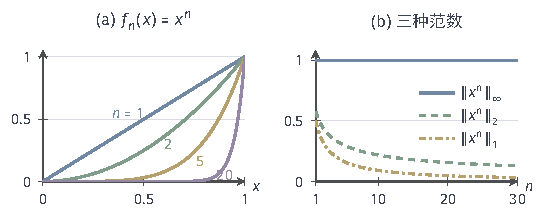
\includegraphics[width=92.3mm]{figures/02-abstract-mathematics/03-function-spaces/tikz/c1-xn-norms/figure.pdf}
  \caption{$x^n$在$[0,1]$上的三种大小。(a)$n=1,2,5,20$时的曲线，函数值集中到右端越来越窄的区间上。(b)三种范数随$n$的变化：$\|x^n\|_\infty=1$，$\|x^n\|_2=(2n+1)^{-1/2}$，$\|x^n\|_1=(n+1)^{-1}$，两个积分范数趋于零，$p=1$下降更快。}
  \label{fig:fs-xn-norms}
\end{figure}

\paragraph{数列空间}
取$X=\mathbb N_+=\{1,2,\ldots\}$与计数测度（每个点的质量为$1$），可测函数就是实数列$x=(x_k)_{k\geq1}$，积分就是求和。此时只有空集是零测集，等价类就是数列本身。$L^p$空间成为
\[
 \ell^p=\Bigl\{x:\ \sum_{k\geq1}|x_k|^p<\infty\Bigr\},\qquad \|x\|_p=\Bigl(\sum_{k\geq1}|x_k|^p\Bigr)^{1/p}.
\]
有限维向量$(x_1,\ldots,x_n)$可以看作后面全为零的数列，$\|x\|_p$就是熟悉的$p$范数，所以$\ell^p$是有限维$p$范数向无限维的自然延伸。数列$x_k=1/k$在$\ell^2$中，因为$\sum_k1/k^2=\pi^2/6$；它不在$\ell^1$中，因为调和级数发散。

\paragraph{平均收敛作为范数收敛}
取概率测度$\mathbb P$，随机变量$Y$的$p$次可积条件就是$\mathbb E|Y|^p<\infty$，范数为$\|Y\|_{L^p(\mathbb P)}=(\mathbb E|Y|^p)^{1/p}$。随机变量的$p$阶平均收敛$\mathbb E|Y_n-Y|^p\to0$因此就是$L^p(\mathbb P)$中的范数收敛。以样本均值为例：设$Y_1,Y_2,\ldots$独立同分布，均值为$m$、方差为$\sigma^2$，则$\bar Y_n=\tfrac1n\sum_{k\leq n}Y_k$满足$\mathbb E(\bar Y_n-m)^2=\sigma^2/n$，即$\|\bar Y_n-m\|_{L^2(\mathbb P)}=\sigma/\sqrt n\to0$。这里只是把已有的平均收敛放进空间结构中，概率收敛的系统理论属于第~\ref{part:probability-spaces}部分，初等的期望与方差计算可参考\BookChapterRef{chap:random-variables}{卷一“随机变量与概率分布”章}。

\subsection{Hölder与Minkowski不等式}
\label{sec:fs-holder-minkowski}

要证明$\|\cdot\|_p$满足三角不等式，需要先控制乘积的积分。设$1<p<\infty$，取$q$满足$\tfrac1p+\tfrac1q=1$，即$q=p/(p-1)$，称$p,q$为\term{共轭指数}（conjugate exponents）。$p=2$时$q=2$；$p=3$时$q=\tfrac32$。

\begin{lemma}[Young不等式]
\label{lem:fs-young}
设$1<p<\infty$，$q$为其共轭指数。对任意$a,b\geq0$，
\[
 ab\leq\frac{a^p}{p}+\frac{b^q}{q},
\]
等号当且仅当$a^p=b^q$。
\end{lemma}

\begin{proof}
固定$b\geq0$，考察$F(s)=\tfrac{s^p}{p}-bs$，$s\geq0$。$F'(s)=s^{p-1}-b$在$s_*=b^{1/(p-1)}$处为零，$s<s_*$时为负、$s>s_*$时为正，所以$F$在$s_*$处取最小值。由$p/(p-1)=q$得$s_*^p=b^q$，于是
\[
 F(s_*)=\frac{b^q}{p}-b\cdot b^{q/p}=\frac{b^q}{p}-b^q=-\frac{b^q}{q},
\]
其中用了$1+q/p=q$。所以$F(a)\geq-b^q/q$，移项即得不等式；等号当且仅当$a=s_*$，即$a^p=b^q$。
\end{proof}

这个不等式有一幅面积图像。共轭条件等价于$(p-1)(q-1)=1$，所以曲线$s=t^{p-1}$也可以写成$t=s^{q-1}$。图~\ref{fig:fs-young-area}中，曲线下方从$0$到$a$的面积是$\int_0^at^{p-1}\,dt=a^p/p$（蓝色），曲线左方从$0$到$b$的面积是$\int_0^bs^{q-1}\,ds=b^q/q$（绿色）。两块区域合起来盖住了矩形$[0,a]\times[0,b]$，所以面积之和不小于$ab$；只有当曲线恰好穿过矩形的右上角，即$b=a^{p-1}$时，两块区域才不多不少地拼成矩形。

\begin{figure}[!htb]
  \centering
  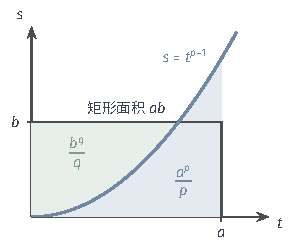
\includegraphics[width=49.6mm]{figures/02-abstract-mathematics/03-function-spaces/tikz/c1-young-area/figure.pdf}
  \caption{Young不等式的面积解释，取$p=3$、$q=\tfrac32$、$a=1$、$b=0.6$。曲线为$s=t^{2}$；蓝色区域面积$a^p/p=\tfrac13$，绿色区域面积$b^q/q\approx0.310$，二者覆盖面积为$ab=0.6$的矩形，多出的部分是曲线在矩形上方的蓝色尖角。}
  \label{fig:fs-young-area}
\end{figure}

\begin{theorem}[Hölder不等式]
\label{thm:fs-holder}
设$1<p<\infty$，$q$为其共轭指数，$f,g$可测。则
\[
 \int_X|fg|\,d\mu\leq\|f\|_p\,\|g\|_q ,
\]
其中右边允许取$+\infty$。特别地，$f\in L^p(\mu)$、$g\in L^q(\mu)$时$fg\in L^1(\mu)$。
\end{theorem}

\begin{proof}
若右边为$+\infty$，无需证明。若$\|f\|_p=0$，则$f=0$几乎处处，$fg=0$几乎处处，左边为零；$\|g\|_q=0$同理。下设$0<\|f\|_p,\|g\|_q<\infty$。在Young不等式中逐点取$a=|f(x)|/\|f\|_p$、$b=|g(x)|/\|g\|_q$，得
\[
 \frac{|f(x)g(x)|}{\|f\|_p\|g\|_q}\leq\frac{|f(x)|^p}{p\|f\|_p^p}+\frac{|g(x)|^q}{q\|g\|_q^q}.
\]
两边积分，右边等于$\tfrac1p+\tfrac1q=1$，再乘以$\|f\|_p\|g\|_q$即得结论。
\end{proof}

归一化这一步的作用是把两个任意大小的函数缩放到“单位大小”，使Young不等式右边的两项积分后恰好凑成$1$。由证明还可以读出等号条件：在每一点都需要$a^p=b^q$，即$|f|^p$与$|g|^q$几乎处处成比例。在$[0,1]$上取$f=x$、$g=x^2$、$p=3$、$q=\tfrac32$：$|f|^p=x^3=|g|^q$，左边$\int_0^1x^3\,dx=\tfrac14$，右边$\|x\|_3\|x^2\|_{3/2}=(\tfrac14)^{1/3}(\tfrac14)^{2/3}=\tfrac14$，等号成立。若取$f=1$、$g=x$、$p=q=2$，左边$\tfrac12$，右边$1\cdot(\tfrac13)^{1/2}\approx0.577$，不等式是严格的。

\begin{theorem}[Minkowski不等式]
\label{thm:fs-minkowski}
设$1\leq p<\infty$，$f,g\in L^p(\mu)$。则$\|f+g\|_p\leq\|f\|_p+\|g\|_p$。因此$(L^p(\mu),\|\cdot\|_p)$是赋范空间。
\end{theorem}

\begin{proof}
$p=1$时，对逐点不等式$|f+g|\leq|f|+|g|$积分即可。设$1<p<\infty$。由第~\ref{sec:fs-lp}小节，$f+g\in L^p$，所以$\int|f+g|^p\,d\mu<\infty$。若它为零，结论平凡，下设它为正。

先把$p$次幂拆成两项：
\[
 |f+g|^p=|f+g|^{p-1}|f+g|\leq|f+g|^{p-1}|f|+|f+g|^{p-1}|g| .
\]
再对每一项用Hölder不等式。由$(p-1)q=p$，$|f+g|^{p-1}$的$q$次积分为$\int|f+g|^p\,d\mu$，所以
\[
 \int|f+g|^{p-1}|f|\,d\mu\leq\Bigl(\int|f+g|^p\,d\mu\Bigr)^{1/q}\|f\|_p ,
\]
第二项同理。两式相加，
\[
 \int|f+g|^p\,d\mu\leq\Bigl(\int|f+g|^p\,d\mu\Bigr)^{1/q}\bigl(\|f\|_p+\|g\|_p\bigr).
\]
左右同除以$(\int|f+g|^p\,d\mu)^{1/q}$（它有限且为正），由$1-\tfrac1q=\tfrac1p$得$\|f+g\|_p\leq\|f\|_p+\|g\|_p$。
\end{proof}

证明中两处条件都不能省：除法要求$\int|f+g|^p\,d\mu$有限且为正，前者来自第~\ref{sec:fs-lp}小节的封闭性估计，后者单独处理。

\paragraph{$0<p<1$时三角不等式失效}
公式$(\int|f|^p\,d\mu)^{1/p}$对$0<p<1$也能计算，但它不是范数。取两点集$\{1,2\}$上的计数测度，$x=(1,0)$、$y=(0,1)$，则$\|x\|_p=\|y\|_p=1$，而
\[
 \|x+y\|_p=(1^p+1^p)^{1/p}=2^{1/p}>2=\|x\|_p+\|y\|_p .
\]
$p=\tfrac12$时左边等于$4$。几何上，范数的单位球$\{v:\|v\|\leq1\}$必定是凸集：若$\|u\|,\|v\|\leq1$，则$\|tu+(1-t)v\|\leq t\|u\|+(1-t)\|v\|\leq1$。图~\ref{fig:fs-unit-balls}画出了平面上$\{|x_1|^p+|x_2|^p\leq1\}$的边界：$p=1,2,\infty$时分别是菱形、圆和正方形，都是凸的；$p=\tfrac12$时边界向内凹，$(1,0)$与$(0,1)$的中点$(\tfrac12,\tfrac12)$满足$2(\tfrac12)^{1/2}\approx1.41>1$，落在集合之外。这正是三角不等式失效的几何表现。

\begin{figure}[!htb]
  \centering
  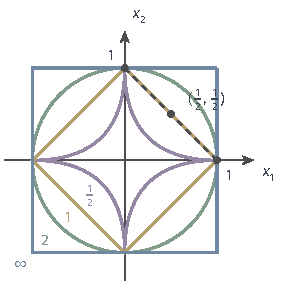
\includegraphics[width=48.6mm]{figures/02-abstract-mathematics/03-function-spaces/tikz/c1-unit-balls/figure.pdf}
  \caption{平面上集合$\{|x_1|^p+|x_2|^p\leq1\}$的边界，曲线旁的数字为$p$；$p=\infty$时为$\max(|x_1|,|x_2|)\leq1$。$p\geq1$时集合是凸的；$p=\tfrac12$时边界内凹，$(1,0)$与$(0,1)$连线的中点$(\tfrac12,\tfrac12)$落在集合外，对应的公式不满足三角不等式。}
  \label{fig:fs-unit-balls}
\end{figure}

\paragraph{$L^2$上的内积}
$p=2$时共轭指数也是$2$，Hölder不等式说明$\int|fg|\,d\mu\leq\|f\|_2\|g\|_2<\infty$，所以
\[
 \langle f,g\rangle=\int_Xfg\,d\mu,\qquad f,g\in L^2(\mu)
\]
有定义，且不依赖代表。对称性与线性来自积分的性质，正定性来自“$\int f^2\,d\mu=0$当且仅当$f=0$几乎处处”。它诱导的范数正是$\|\cdot\|_2$。因此$L^2(\mu)$是内积空间；等第~\ref{sec:fs-lp-completeness}小节证明完备性后，它就是Hilbert空间。

\subsection{$L^\infty$与本质上界}
\label{sec:fs-linfty}

最大偏差也要适应“忽略零测集”的约定。普通上确界会被单个点的值左右，而等价类中的代表可以在零测集上任意改值，所以需要一个只看“几乎处处”的上界。

\begin{definition}[本质上确界与$L^\infty$]
\label{def:fs-linfty}
对可测函数$f$，定义
\[
 \|f\|_\infty=\inf\{M\geq0:\ |f|\leq M\ \text{在}\ \mu\ \text{下几乎处处成立}\},
\]
称为$|f|$的\term{本质上确界}（essential supremum），约定空集的下确界为$+\infty$。本质上确界有限的可测函数称为本质有界的；其几乎处处等价类全体记为$L^\infty(\mu)$。
\end{definition}

先看下确界能否取到。记$M_0=\|f\|_\infty<\infty$，对每个正整数$k$，集合$\{|f|>M_0+1/k\}$是零测集；它们的并$\{|f|>M_0\}$是可数个零测集之并，仍为零测集。所以$|f|\leq\|f\|_\infty$几乎处处成立，下确界是可以达到的。由此也看出数值不依赖代表：若$g\sim_\mu f$，则$\{|g|>M\}\subseteq\{|f|>M\}\cup\{f\neq g\}$，两类函数的本质上界相同。

本质上确界与普通上确界可以相差很远。在$[0,1]$上取Lebesgue测度，令$f(x)=x$，但把$f(\tfrac12)$改为$2$。普通上确界是$2$，而$|f|\leq1$只在单点$\{\tfrac12\}$外成立，所以本质上确界是$1$，如图~\ref{fig:fs-essential-sup}所示。更极端地，有理点示性函数$\mathbf 1_{\mathbb Q\cap[0,1]}$的普通上确界是$1$，本质上确界是$0$，因为有理点只有可数个，组成零测集。这也说明：$\|f\|_\infty\leq M$只保证某个零测集之外处处$|f|\leq M$，并不保证类中任意一个代表在每一点都受这个界控制。若$f$在区间上连续，则$\{|f|>M\}$是开集，非空即有正测度，所以连续函数的本质上确界等于普通上确界。

\begin{figure}[!htb]
  \centering
  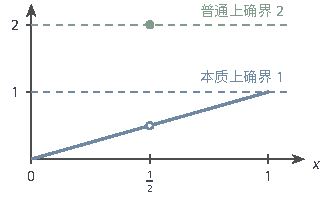
\includegraphics[width=56.1mm]{figures/02-abstract-mathematics/03-function-spaces/tikz/c1-essential-sup/figure.pdf}
  \caption{本质上确界忽略零测集。$[0,1]$上取Lebesgue测度，$f(x)=x$，只把$f(\tfrac12)$改为$2$（绿点，空心圈为原值）。普通上确界被这一个点抬到$2$；单点测度为零，本质上确界仍为$1$。}
  \label{fig:fs-essential-sup}
\end{figure}

\paragraph{范数公理与积分配对}
$\|\cdot\|_\infty$在$L^\infty(\mu)$上是范数，论证的关键是把例外集合并成一个零测集。正定性：若$\|f\|_\infty=0$，由上一段$|f|\leq0$几乎处处，即$f=0$几乎处处。齐次性由$|cf|=|c||f|$得到。三角不等式：$|f|\leq\|f\|_\infty$在零测集$N_f$外成立，$|g|\leq\|g\|_\infty$在零测集$N_g$外成立，于是在$N_f\cup N_g$之外$|f+g|\leq\|f\|_\infty+\|g\|_\infty$，例外集仍是零测集。

$L^\infty$与$L^1$之间有一个自然的积分配对，它是Hölder不等式在端点$p=1$、$q=\infty$的形式：由$|fg|\leq|f|\,\|g\|_\infty$几乎处处成立并积分，
\[
 \int_X|fg|\,d\mu\leq\|f\|_1\,\|g\|_\infty .
\]
约定$\tfrac1\infty=0$后，Hölder不等式对所有共轭指数对$1\leq p\leq\infty$都成立。第~\ref{sec:lfo-lp-dual}小节将从这个配对出发研究$L^p$上的线性泛函。

\paragraph{有界数列空间}
取$\mathbb N_+$上的计数测度，只有空集零测，本质上确界就是普通上确界，得到有界数列空间$\ell^\infty=\{x:\sup_k|x_k|<\infty\}$。常数列$(1,1,1,\ldots)$在$\ell^\infty$中，却不在任何$\ell^p$（$p<\infty$）中。第~\ref{sec:fs-density-separability}小节将看到，$\ell^\infty$与$L^\infty([0,1])$都“太大”，无法用可数个元素逼近；第~\ref{sec:lfo-weak-star}小节则会在$L^\infty$上使用另一种更弱的收敛。

\subsection{积分空间的完备性}
\label{sec:fs-lp-completeness}

现在回答本节开头的问题：积分误差下的Cauchy列是否一定有极限？下面的定理对所有$1\leq p\leq\infty$给出肯定回答，但有限$p$与$p=\infty$的证明方式不同，不能把一个套到另一个上。

\begin{theorem}[积分空间的完备性]
\label{thm:fs-lp-complete}
对任意测度空间与$1\leq p\leq\infty$，$L^p(\mu)$是Banach空间。特别地，$L^2(\mu)$是Hilbert空间。
\end{theorem}

\begin{proof}
先设$1\leq p<\infty$，$(f_n)$是$L^p$中的Cauchy列。证明分五步：抽出快速子列，构造控制函数，定义候选极限，证明子列收敛，最后回到整列。

第一步，抽取相邻差可求和的子列。由Cauchy条件，可以递归地取$n_1<n_2<\cdots$，使$m,n\geq n_k$时$\|f_n-f_m\|_p<2^{-k}$。于是$\|f_{n_{k+1}}-f_{n_k}\|_p<2^{-k}$，$\sum_k\|f_{n_{k+1}}-f_{n_k}\|_p<\infty$。取定各项的可测代表。

第二步，构造控制函数。令
\[
 S_m=|f_{n_1}|+\sum_{k=1}^m|f_{n_{k+1}}-f_{n_k}|,\qquad S=\lim_{m\to\infty}S_m\in[0,\infty].
\]
由Minkowski不等式，$\|S_m\|_p\leq\|f_{n_1}\|_p+\sum_k\|f_{n_{k+1}}-f_{n_k}\|_p=:C<\infty$，界与$m$无关。$S_m^p$逐点单调上升到$S^p$，由单调收敛定理，$\int S^p\,d\mu=\lim_m\int S_m^p\,d\mu\leq C^p$。所以$S\in L^p$，特别地$S<\infty$几乎处处。

第三步，定义候选极限。在$\{S<\infty\}$上，级数$f_{n_1}+\sum_k(f_{n_{k+1}}-f_{n_k})$绝对收敛，其部分和恰为$f_{n_{k+1}}$；令$f$为其和，在零测集$\{S=\infty\}$上令$f=0$。$f$是可测函数列的几乎处处极限，因而可测；$|f|\leq S$，所以$f\in L^p$。至此子列$f_{n_j}\to f$几乎处处。

第四步，证明子列依范数收敛。固定$j$，在$\{S<\infty\}$上$f-f_{n_j}=\lim_{m\to\infty}(f_{n_m}-f_{n_j})$。由Fatou引理与Minkowski不等式，
\[
 \int|f-f_{n_j}|^p\,d\mu\leq\liminf_{m\to\infty}\int|f_{n_m}-f_{n_j}|^p\,d\mu
 \leq\Bigl(\sum_{k\geq j}\|f_{n_{k+1}}-f_{n_k}\|_p\Bigr)^p,
\]
右边是收敛级数的尾和的$p$次方，趋于零。所以$\|f_{n_j}-f\|_p\to0$。

第五步，回到整列。给定$\varepsilon>0$，取$N$使$m,n\geq N$时$\|f_n-f_m\|_p<\varepsilon$，再取$j$使$n_j\geq N$且$\|f_{n_j}-f\|_p<\varepsilon$。则$n\geq N$时$\|f_n-f\|_p\leq\|f_n-f_{n_j}\|_p+\|f_{n_j}-f\|_p<2\varepsilon$。

再设$p=\infty$。取$L^\infty$中的Cauchy列$(f_n)$的代表。对每对$m,n$，$|f_n-f_m|\leq\|f_n-f_m\|_\infty$在某个零测集$E_{m,n}$之外成立。令$E=\bigcup_{m,n}E_{m,n}$，它是可数个零测集之并，仍为零测集。在$X\setminus E$上，所有这些不等式同时成立，所以$(f_n)$在$X\setminus E$上一致Cauchy。与定理~\ref{thm:fs-continuous-complete}的前两步相同，$f_n$在$X\setminus E$上一致收敛到某个函数$f$；在$E$上令$f=0$。$f$是可测函数列在$X\setminus E$上的逐点极限，因而可测；$\sup_{x\notin E}|f_n(x)-f(x)|\to0$给出$\|f_n-f\|_\infty\to0$。取$n_0$使$\|f_{n_0}-f\|_\infty\leq1$，则$\|f\|_\infty\leq\|f_{n_0}\|_\infty+1<\infty$，所以$f\in L^\infty$。

最后，$L^2$的范数由内积诱导，完备后即为Hilbert空间。
\end{proof}

两种证明的差别值得对照。有限$p$的论证没有一致性可用，只能先抽子列，借$S\in L^p$得到几乎处处收敛，再用Fatou引理把逐点信息转为积分信息；$p=\infty$的论证则把可数个例外集合并成一个零测集，在其补集上做一致收敛，与连续函数空间的证明如出一辙。

证明的前三步还给出了一个单独有用的结论，第~\ref{sec:fs-convergence-modes}小节比较收敛方式时会用到。

\begin{theorem}[范数收敛的几乎处处收敛子列]
\label{thm:fs-ae-subsequence}
设$1\leq p<\infty$，$f_n\to f$在$L^p(\mu)$中成立。则存在子列$(f_{n_k})$使$f_{n_k}\to f$几乎处处成立。
\end{theorem}

\begin{proof}
收敛列是Cauchy列。定理~\ref{thm:fs-lp-complete}证明的前四步构造出子列和函数$\tilde f$，使$f_{n_k}\to\tilde f$几乎处处且在$L^p$中成立。$L^p$极限唯一，所以$\tilde f=f$几乎处处。
\end{proof}

回到斜坡例子。在$L^2([-1,1])$中，$\operatorname{sgn}$的等价类是一个合法元素，并且
\[
 \|g_n-\operatorname{sgn}\|_2^2=2\int_0^{1/n}(1-nx)^2\,dx=\frac{2}{3n}\to0 .
\]
所以在$L^2$中，斜坡列有了极限。$\operatorname{sgn}$在$0$处取什么值无关紧要，这正是取等价类的用意。
